\documentclass{beamer}


\usetheme{Madrid}
\usecolortheme{default}


% --- PREAMBLE: PACKAGES AND DOCUMENT INFO ---
\usepackage[utf8]{inputenc}
\usepackage[T1]{fontenc}
\usepackage{amsmath}
\usepackage{amsfonts}
\usepackage{amssymb}
\usepackage{tikz}
\usepackage{hyperref}
\usetikzlibrary{positioning}
\usepackage{subcaption}

\usetikzlibrary{arrows.meta}
\tikzset{
    dot/.style={circle, fill, inner sep=1.5pt}, % 定义格点的样式
    main plot/.style={scale=0.7, font=\small} % 定义每个子图的通用样式
}

\usefonttheme{professionalfonts} % 允许更自由的字体尺寸设置
\AtBeginDocument{\small} % 在文档开始时全局应用 small 字体

% --- 全局行间距设置 ---
\usepackage{setspace}
\setstretch{1.2} % 全局设置行间距为1.2倍

\newcommand{\ket}[1]{\left| #1 \right\rangle}
\newcommand{\vev}[1]{\left\langle #1 \right\rangle}


% --- Fill in your information here ---
\title[The \texorpdfstring{$\widetilde{SL}_{2}(\mathbb{R})$}{Sl(2,R)} WZW Model]{Degenerate Representations and Fusion Rules in the $\widetilde{SL}_{2}(\mathbb{R})$ WZW Model}

% The \author command can hold your name.
% The optional [short name] is for the footer if your name is long.
\author[Hexuan Li]{Hexuan Li}

% The \institute command can hold your university and advisor information.
\institute[École Polytechnique]
{
  
  Advisor: Prof. Sylvain Ribault
}

% The \date command sets the date on the title page. \today is automatic.
\date{\today}


% --- BEGIN DOCUMENT ---
\begin{document}

% --- TITLE PAGE FRAME ---
% The [plain] option removes the header and footer for a clean title page.
\begin{frame}[plain]
  \titlepage
\end{frame}

\begin{frame}{Contents}
  \tableofcontents
\end{frame}

\section{Introduction}

\begin{frame}{Introduction}

  \begin{center}
  % node distance 定义了两个节点边框之间的距离
  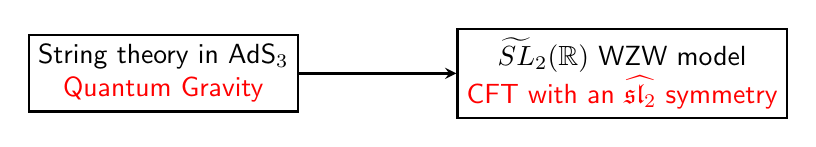
\begin{tikzpicture}[node distance=2cm] 
      
      \node[draw, thick, font=\sffamily, align=center] (c1) {String theory in AdS${}_{3}$ \\ \textcolor{red}{Quantum Gravity}};

      \node[draw, thick, font=\sffamily, right=of c1, align=center] (c2) {$\widetilde{SL}_{2}(\mathbb{R})$ WZW model\\ \textcolor{red}{CFT with an $\widehat{\mathfrak{sl}_{2}}$ symmetry}};

      \draw[-stealth, thick] (c1) -- (c2);
      
  \end{tikzpicture}
  \end{center}

  The crossing symmetry equation: 
  \begin{equation*}
      \sum_{k \in \mathcal{S}} 
      \vcenter{\hbox{
      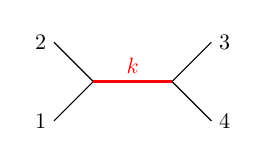
\begin{tikzpicture}[
          scale=0.5, % 调整图形整体大小
          every node/.style={scale=0.8} % 调整节点(数字)大小
      ]
        % s-channel diagram
        % 绘制外部的四条腿和标签
        \draw (0,0) -- (-1,1)   node[left]  {2};
        \draw (0,0) -- (-1,-1)  node[left]  {1};
        \draw (2,0) -- (3,1)    node[right] {3};
        \draw (2,0) -- (3,-1)   node[right] {4};
        % 绘制中间的传播子和标签
        \draw[red,thick] (0,0) -- (2,0)    node[midway, above] {$k$};
      \end{tikzpicture}
    }}
    = \sum_{k' \in \mathcal{T}}
    \vcenter{\hbox{
      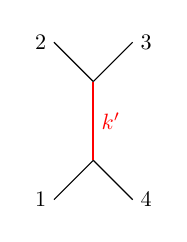
\begin{tikzpicture}[
          scale=0.5,
          every node/.style={scale=0.8}
      ]
        % t-channel diagram
        % 绘制外部的四条腿和标签
        \draw (0,0) -- (-1,-1)  node[left]  {1};
        \draw (0,0) -- (1,-1)   node[right] {4};
        \draw (0,2) -- (-1,3)   node[left]  {2};
        \draw (0,2) -- (1,3)    node[right] {3};
        % 绘制中间的传播子和标签
        \draw[red,thick] (0,0) -- (0,2)    node[midway, right] {$k'$};
      \end{tikzpicture}
    }}
    \end{equation*}

    \begin{block}{}
      \begin{center}
        Degenerate representations $\Longrightarrow $ Finite many terms
      \end{center}
    \end{block}
\end{frame}

\section{\texorpdfstring{$\widetilde{SL}_{2}(\mathbb{R})$}{SL(2,R)} WZW model: Review}

\begin{frame}{Symmetry algebra}
  \begin{itemize}
    \item The $\mathfrak{sl}_{2}$ algebra: 
      \begin{equation*}
        \left[J^{0}, J^{\pm}\right] = \pm J^{\pm}, \quad \left[J^{+}, J^{-}\right] = 2 J^{0}.
      \end{equation*}
    \item The $\widehat{\mathfrak{sl}_{2}}$ algebra are defined by:
      \begin{equation*}
          \left[ J^{a}_{m}, J^{b}_{n} \right] = f^{ab}_{c} J^{c}_{m+n} + k m K^{ab} \delta_{m+n,0}, \quad a,b \in \{0,\pm\} \, ,\,  m,n \in \mathbb{Z}
      \end{equation*}
      where $k$ is a constant, and $K^{ab} = \frac{1}{2} f^{ac}_{d}f^{bd}_{c}$ is the Killing tensor.
    \item The Sugawara construction of the dilation operator:
      \begin{equation*}
        L_{0} = \frac{K_{ab}}{2(k-2)} \left(J^{a}_{0}J^{b}_{0} + 2\sum_{m > 0 } J^{a}_{-m} J^{b}_{m}\right).
      \end{equation*}
  \end{itemize}
\end{frame}

\begin{frame}{Irreducible representations of \texorpdfstring{$\mathfrak{sl}_{2}$}{Lg}}

  We characterize different representations by the spin $j$ and the eigenvalue $m$ of $J^{0}_{0}$:
  \begin{itemize}
    \item $\mathcal{C}^{j}_{\alpha}$: $j \in -\frac{1}{2} + i \mathbb{R}_{+}$, $m \in \alpha + \mathbb{Z}$.
    
      \begin{center}
      % node distance 定义了两个节点边框之间的距离
      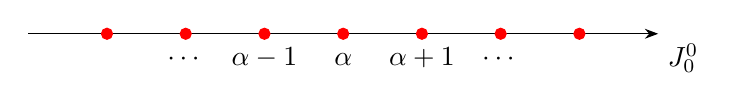
\begin{tikzpicture}
          % --- 1. 使用高级循环,同时绘制点和下方的坐标标签 ---
          % 循环的格式是: \x / \labelText
          % \x 是横坐标,\labelText 是要显示的标签文本
          \draw[-{Stealth}] (-4, 0) -- (4, 0) node[anchor=north west] {$J_0^0$};

          \foreach \x / \labelText in {
              -3/{},
              -2/{\cdots}, 
              -1/{\alpha-1}, 
              0/{\alpha}, 
              1/{\alpha+1}, 
              2/{\cdots},
              3/{}
          } {
              \filldraw[red] (\x, 0) circle (2pt);
              
              \node[anchor=base] at (\x, -0.4) {$\labelText$};
          }

      \end{tikzpicture}

      \end{center}

    \item $\mathcal{E}^{j}$: $j \in \mathbb{N}/2$, $m \in \left\{-j, -j+1, \cdots, j-1, j \right\}$.
    \begin{center}
      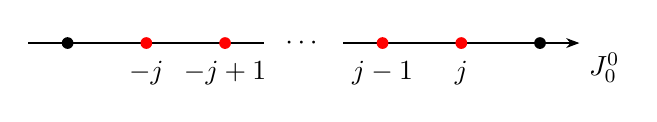
\begin{tikzpicture}[
          dot/.style={circle, fill, inner sep=1.5pt}
      ]

          \draw (-3.5, 0) -- (-0.5, 0);

          \draw[-{Stealth}] (0.5, 0) -- (3.5, 0) node[anchor=north west] {$J^{0}_{0}$};

          \node[dot, black] at (-3, 0) {}; 

          \node[dot, red] at (-2, 0) {}; 
          \node[below=3pt] at (-2, 0) {$-j$}; 
          
          \node[dot, red] at (-1, 0) {}; 
          \node[below=3pt] at (-1, 0) {$-j+1$}; 

          \node[dot, red] at (1, 0) {}; 
          \node[below=3pt] at (1, 0) {$j-1$};

          \node[dot, red] at (2, 0) {}; 
          \node[below=3pt] at (2, 0) {$j$};

          \node[dot, black] at (3, 0) {}; 

          \node at (0, 0) {$\cdots$};
          
      \end{tikzpicture}
    \end{center}
    $\mathcal{E}^{j}$ is a level 0 degenerate representation, with the following null vector: 
    \begin{equation*}
      J^{-}_{0} \ket{j,-j} = 0.
    \end{equation*}
  \end{itemize}
\end{frame}


\begin{frame}{Affine highest-weight representations of \texorpdfstring{$\widehat{\mathfrak{sl}_{2}}$}{Lg}}

  \begin{center}
  % node distance 定义了两个节点边框之间的距离
  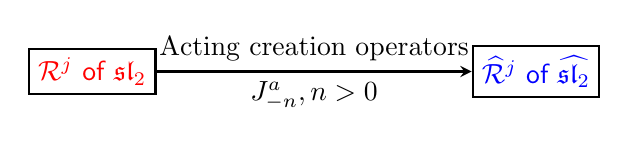
\begin{tikzpicture}[node distance=4cm] 
      
      \node[draw, thick, font=\sffamily, align=center] (c1) {\textcolor{red}{$\mathcal{R}^{j}$ of $\mathfrak{sl}_{2}$}};

      \node[draw, thick, font=\sffamily, right=of c1, align=center] (c2) {\textcolor{blue}{$\widehat{\mathcal{R}}^{j}$ of $\widehat{\mathfrak{sl}_{2}}$}};

      \draw[-stealth, thick] (c1) -- node[above] {Acting creation operators} node[below] {$J^{a}_{-n}, n>0$} (c2);
      
  \end{tikzpicture}
  \end{center}
\begin{figure}
    \centering
    \def\tikzscale{0.5} 

    \begin{subfigure}[b]{0.48\textwidth}
        \centering
        \begin{tikzpicture}[scale=\tikzscale, font=\small] % 使用定义的 scale
            \def\xmin{-4.5} \def\xmax{4.5} \def\ymin{-2.5} \def\ymax{4.5}
            \clip (\xmin-1, \ymin) rectangle (\xmax+1, \ymax+1);
            \fill[violet!20] (\xmin, 0) rectangle (\xmax, \ymax);
            \draw[-{Stealth[]}] (\xmin, 0) -- (\xmax, 0) node[anchor=north west, xshift=-10pt] {$J_0^0$};
            \draw[-{Stealth[]}] (0, \ymin) -- (0, \ymax) node[anchor=south east] {$L_0$};
            \foreach \x in {-4,...,4} {\foreach \y in {-2,-1} {\node[dot] at (\x+0.2,\y) {};}}
            \foreach \x in {-4,...,4} {\foreach \y in {0} {\node[dot, red] at (\x+0.2,\y) {};}}
            \foreach \x in {-4,...,4} {\foreach \y in {1,2,3,4} {\node[dot, blue] at (\x+0.2,\y) {};}}
            \node[draw, fill=white, rounded corners=2pt, align=left, anchor=north east, font=\tiny] at (\xmax-0.2, \ymax-0.2) {
                \begin{tabular}{rl}\tikz\fill[violet!20](0,0)rectangle(0.2,0.2);&Allowed states\end{tabular}};
        \end{tikzpicture}
        \caption{$\widehat{\mathcal{C}}^{j}_{\alpha}$}
        \label{fig:C}
    \end{subfigure}
    \hfill
    \begin{subfigure}[b]{0.48\textwidth}
        \centering
        \begin{tikzpicture}[scale=\tikzscale, font=\small] 
            \def\xmin{-4.5} \def\xmax{4.5} \def\ymin{-2.5} \def\ymax{4.5}
            \clip (\xmin-1, \ymin) rectangle (\xmax+1, \ymax+1);
            \fill[violet!20] (\xmin, -\xmin-1) -- (-1, 0) -- (1, 0) -- (\xmax, \xmax-1) -- (\xmax, \ymax) -- (\xmin, \ymax) -- cycle;
            \draw[-{Stealth[]}] (\xmin, 0) -- (\xmax, 0) node[anchor=north west, xshift=-10pt] {$J_0^0$};
            \draw[-{Stealth[]}] (0, \ymin) -- (0, \ymax) node[anchor=south east] {$L_0$};
            \foreach \x in {-4,...,4} {\foreach \y in {-2,-1} {\node[dot] at (\x,\y) {};}}
            \foreach \x in {-4,-3,-2} {\foreach \y in {0} {\node[dot] at (\x,\y) {};}}
            \foreach \x in {-1,0,1} {\foreach \y in {0} {\node[dot, red] at (\x,\y) {};}}
            \foreach \x in {2,3,4} {\foreach \y in {0} {\node[dot] at (\x,\y) {};}}
            
            \foreach \x in {-4,-3} {\foreach \y in {1} {\node[dot] at (\x,\y) {};}}
            \foreach \x in {-2,...,2} {\foreach \y in {1} {\node[dot, blue] at (\x,\y) {};}}
            \foreach \x in {3,4} {\foreach \y in {1} {\node[dot] at (\x,\y) {};}}

            \foreach \x in {-4} {\foreach \y in {2} {\node[dot] at (\x,\y) {};}}
            \foreach \x in {-3,...,3} {\foreach \y in {2} {\node[dot, blue] at (\x,\y) {};}}
            \foreach \x in {4} {\foreach \y in {2} {\node[dot] at (\x,\y) {};}}
            
            \foreach \x in {-4,...,4} {\foreach \y in {3,4} {\node[dot, blue] at (\x,\y) {};}}
            \node[draw, fill=white, rounded corners=2pt, align=left, anchor=north east, font=\tiny] at (\xmax-0.2, \ymax-0.2) {
                \begin{tabular}{rl}\tikz\fill[violet!20](0,0)rectangle(0.2,0.2);&Allowed states\end{tabular}};
        \end{tikzpicture}
        \caption{$\widehat{\mathcal{E}}^{j}$}
        \label{fig:E}
    \end{subfigure}
    
\end{figure}
\end{frame}

\begin{frame}{Affine highest-weight representations of \texorpdfstring{$\widehat{\mathfrak{sl}_{2}}$}{Lg}}

  \begin{center}
  % node distance 定义了两个节点边框之间的距离
  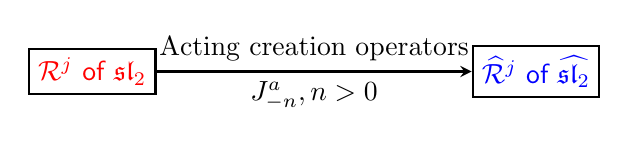
\begin{tikzpicture}[node distance=4cm] 
      
      \node[draw, thick, font=\sffamily, align=center] (c1) {\textcolor{red}{$\mathcal{R}^{j}$ of $\mathfrak{sl}_{2}$}};

      \node[draw, thick, font=\sffamily, right=of c1, align=center] (c2) {\textcolor{blue}{$\widehat{\mathcal{R}}^{j}$ of $\widehat{\mathfrak{sl}_{2}}$}};

      \draw[-stealth, thick] (c1) -- node[above] {Acting creation operators} node[below] {$J^{a}_{-n}, n>0$} (c2);
      
  \end{tikzpicture}
  \end{center}

\begin{figure}
    \centering
    \def\tikzscale{0.5} 

        \begin{subfigure}[b]{0.48\textwidth}
        \centering
        \begin{tikzpicture}[scale=\tikzscale, font=\small] % 使用定义的 scale
            \def\xmin{-4.5} \def\xmax{4.5} \def\ymin{-2.5} \def\ymax{4.5}
            \clip (\xmin-1, \ymin) rectangle (\xmax+1, \ymax+1);
            \fill[violet!20] (\xmin, 0) rectangle (\xmax, \ymax);
            \draw[-{Stealth[]}] (\xmin, 0) -- (\xmax, 0) node[anchor=north west, xshift=-10pt] {$J_0^0$};
            \draw[-{Stealth[]}] (0, \ymin) -- (0, \ymax) node[anchor=south east] {$L_0$};
            \foreach \x in {-4,...,4} {\foreach \y in {-2,-1} {\node[dot] at (\x+0.2,\y) {};}}
            \foreach \x in {-4,...,4} {\foreach \y in {0} {\node[dot, red] at (\x+0.2,\y) {};}}
            \foreach \x in {-4,...,4} {\foreach \y in {1,2,3,4} {\node[dot, blue] at (\x+0.2,\y) {};}}

            \node[dot, green] at (0.2, 1) {};
            \node[draw, fill=white, rounded corners=2pt, align=left, anchor=north east, font=\tiny] at (\xmax-0.2, \ymax-0.2) {
            \begin{tabular}{rl}\tikz\fill[violet!20](0,0)rectangle(0.2,0.2);&Allowed states\\ \tikz\fill[green] (0,0) circle (3pt) ;&Null vector\\ \end{tabular}};

        \end{tikzpicture}
        \caption{$\widehat{\mathcal{C}}^{j}_{\alpha}$}
        \label{fig:C1}
    \end{subfigure}
    \hfill
    \begin{subfigure}[b]{0.48\textwidth}
        \centering
        \begin{tikzpicture}[scale=\tikzscale, font=\small] 
            \def\xmin{-4.5} \def\xmax{4.5} \def\ymin{-2.5} \def\ymax{4.5}
            \clip (\xmin-1, \ymin) rectangle (\xmax+1, \ymax+1);
            \fill[violet!20] (\xmin, -\xmin-1) -- (-1, 0) -- (1, 0) -- (\xmax, \xmax-1) -- (\xmax, \ymax) -- (\xmin, \ymax) -- cycle;
            \draw[-{Stealth[]}] (\xmin, 0) -- (\xmax, 0) node[anchor=north west, xshift=-10pt] {$J_0^0$};
            \draw[-{Stealth[]}] (0, \ymin) -- (0, \ymax) node[anchor=south east] {$L_0$};
            \foreach \x in {-4,...,4} {\foreach \y in {-2,-1} {\node[dot] at (\x,\y) {};}}
            \foreach \x in {-4,-3,-2} {\foreach \y in {0} {\node[dot] at (\x,\y) {};}}
            \foreach \x in {-1,0,1} {\foreach \y in {0} {\node[dot, red] at (\x,\y) {};}}
            \foreach \x in {2,3,4} {\foreach \y in {0} {\node[dot] at (\x,\y) {};}}
            
            \foreach \x in {-4,-3} {\foreach \y in {1} {\node[dot] at (\x,\y) {};}}
            \foreach \x in {-2,...,2} {\foreach \y in {1} {\node[dot, blue] at (\x,\y) {};}}
            \foreach \x in {3,4} {\foreach \y in {1} {\node[dot] at (\x,\y) {};}}

            \foreach \x in {-4} {\foreach \y in {2} {\node[dot] at (\x,\y) {};}}
            \foreach \x in {-3,...,3} {\foreach \y in {2} {\node[dot, blue] at (\x,\y) {};}}
            \foreach \x in {4} {\foreach \y in {2} {\node[dot] at (\x,\y) {};}}
            
            \foreach \x in {-4,...,4} {\foreach \y in {3,4} {\node[dot, blue] at (\x,\y) {};}}
            \node[draw, fill=white, rounded corners=2pt, align=left, anchor=north east, font=\tiny] at (\xmax-0.2, \ymax-0.2) {
                \begin{tabular}{rl}\tikz\fill[violet!20](0,0)rectangle(0.2,0.2);&Allowed states\end{tabular}};
        \end{tikzpicture}
        \caption{$\widehat{\mathcal{E}}^{j}$}
    \end{subfigure}
    
\end{figure}
\end{frame}

\begin{frame}{Spectral flow}
  \begin{itemize}
    \item The spectral flow is a family $(\rho_{\omega})_{\omega \in \mathbb{Z}}$ of automorphisms of $\widehat{\mathfrak{sl}_{2}}$: 
      \begin{equation*}
          \begin{aligned}
              \rho_{\omega}(J^{\pm}_{m}) & = J^{\pm}_{m \pm \omega},\\
              \rho_{\omega}(J^{0}_{m}) & = J^{0}_{m} + \frac{1}{2} k \omega \delta_{m,0}.
          \end{aligned}
      \end{equation*}
    \item The spectral flowed representation $\rho_{\omega}\left(\widehat{\mathcal{R}}\right)$ is related to
     $\widehat{\mathcal{R}}$ through
     \begin{equation*}
        J^{a}_{n} \left|v, \omega \right\rangle = \rho_{-\omega}\left(J^{a}_{n}\right) \left|v \right\rangle.
     \end{equation*}
  \end{itemize}
\end{frame}

\section{Fusion rules: Results}

\begin{frame}{My contributions}
  \begin{itemize}
    \item The structure of spectral flowed degenerate representation
        \begin{itemize}
          \item Spectral flowed vacuum representation
        \end{itemize}
    \item Fusion rules with degenerate representations
        \begin{itemize}
          \item level 0 
          \item level 1 
        \end{itemize}
  \end{itemize}
\end{frame}

\begin{frame}{Fusion rules}
  \begin{itemize}
    \item The fusion rules are determined from the OPE 
          \begin{equation*}
            \begin{aligned}
              \phi^{\ket{j_{1},m_{1},\omega_{1}}} & (z_{1})\phi^{\ket{j_{2},m_{2}, \omega_{2}}}(z_{2}) \sim \\
               \sum_{j_{3},\omega_{3}} 
              &\left\langle  \phi^{\ket{j_{1},m_{1},\omega_{1}}}(z_{1}) \phi^{\ket{j_{2},m_{2}, \omega_{2}}}(z_{2}) \left(\phi^{\ket{j_{3},m_{3},\omega_{3}}}(z_{3}) \right)^{\dagger}\right\rangle \phi^{\ket{j_{3},m_{3},\omega_{3}}}(z_{3}).
            \end{aligned}
          \end{equation*}
          \begin{equation*}
              \vev{\phi^{\ket{j_{1},m_{1},\omega_{1}}}(z_{1}) \phi^{\ket{j_{2},m_{2}, \omega_{2}}}(z_{2}) \left(\phi^{\ket{j_{3},m_{3},\omega_{3}}}(z_{3}) \right)^{\dagger}} 
            \neq 0
          \end{equation*}
          \begin{equation*}
             \Longleftrightarrow \widehat{\mathcal{R}}^{j_{1},\omega_{1}} \times \widehat{\mathcal{R}}^{j_{2},\omega_{2}} \supset \widehat{\mathcal{R}}^{j_{3},\omega_{3}}
          \end{equation*}
    \item The fusion rules involving degenerate representations is constrained by the null vector equations:
          \begin{equation*}
            \hat{N} \ket{j,m,\omega} = 0 \Longrightarrow \vev{\hat{N} \phi^{\ket{j,m,\omega}}(z)\, \prod_{i} \phi^{\ket{j_{i},m_{i},\omega_{i}}} (z_{i} )} = 0.
          \end{equation*}
  \end{itemize}
\end{frame}

\begin{frame}{Spectral flowed vacuum representation}
  \begin{itemize}
    \item $\rho_{\pm 1} \left(\widehat{\mathcal{E}}^{0}\right)$ is a level 1 degenerate representation, with the corresponding null vector:
      \begin{equation*}
        J^{\mp 1}_{-1} \ket{k/2,\mp k/2} = 0.
      \end{equation*}
    \item The corresponding null vector equation:
      \begin{equation*}
          \vev{J^{\pm}_{-1} \phi^{\ket{k/2,\pm k/2 } }(z_{1} ) \phi ^{\ket{j_{2},m_{2}}} ( z_{2})
            \phi ^{\ket{j_{3},m_{3}, \mp 1}} ( z_{3} ) }= 0,
      \end{equation*}
      \begin{equation*}
          \Longrightarrow j_{2}(j_{2}+1) = j_{3}(j_{3}+1)
      \end{equation*}
    \item We have the following fusion rule:
      \begin{equation*}
          \rho_{\pm 1} \left( \widehat{\mathcal{E}}^{0} \right) \times \widehat{\mathcal{R}}^{j} = \rho_{\pm 1} \left( \widehat{\mathcal{R}}^{j} \right).
      \end{equation*}
  \end{itemize}
\end{frame}

\begin{frame}{Fusion rules with spectral flowed representations}
  \begin{itemize}
    \item We conjecture that the spectral flow commutes with fusion,  
      \begin{equation*}
          \rho_{\omega_{1}} \left(\widehat{\mathcal{R}}^{j_{1}}\right) \times \rho_{\omega_{2}} \left(\widehat{\mathcal{R}}^{j_{2}}\right) = \rho_{\omega_{1} + \omega_{2}} \left(\widehat{\mathcal{R}}^{j_{1}} \times\widehat{\mathcal{R}}^{j_{2}}\right). \label{SpecFus}
      \end{equation*}
    \item The fusion rule with $\rho_{\pm 1} \left(\widehat{\mathcal{E}}^{0}\right)$ proves the simplest case:
      \begin{equation*}
        \begin{aligned}
          \rho_{\pm 1} \left(\widehat{\mathcal{R}}^{j_{1}}\right) \times \widehat{\mathcal{R}}^{j_{2}} 
          &= \left(\rho_{\pm 1} \left( \widehat{\mathcal{E}}^{0} \right) \times \widehat{\mathcal{R}}^{j_{1}} \right) \times \widehat{\mathcal{R}}^{j_{2}}\\
          &= \rho_{\pm 1} \left( \widehat{\mathcal{E}}^{0} \right) \times \left( \widehat{\mathcal{R}}^{j_{1}}  \times \widehat{\mathcal{R}}^{j_{2}} \right) \\
          &= \rho_{\pm 1} \left(\widehat{\mathcal{R}}^{j_{1}} \times \widehat{\mathcal{R}}^{j_{2}} \right).
        \end{aligned}
      \end{equation*}
  \end{itemize}
\end{frame}

\begin{frame}{Level 1 degenerate representations}
  \begin{itemize}
    \item Degenerate representations $\widehat{\mathcal{R}}^{\vev{r,s}}$ are labeled by two integers $r$ and $s$ for $r \geq 0, s\geq 1 $, with 
    the corresponding null vector at level $N = rs$.
      \begin{equation*}
          j_{\vev{r,s}} = \frac{s-1}{2} - \frac{k+2}{2} r.
      \end{equation*}
    \item The null vector for level 1 degenerate representation is given by the following null operator:
      \begin{equation*}
          \hat{N}^{c} = K_{ab} J^{a}_{-1} J^{b}_{0} J^{c}_{0} + j_{\vev{1,1}} f^{c}_{ab} J^{a}_{-1} J^{b}_{0} - 2 j^{2}_{\vev{1,1}} J^{c}_{-1}.
      \end{equation*}
  \end{itemize}
\end{frame}

\begin{frame}{Fusion with level 1 degenerate representation}
  \begin{itemize}
    \item Let's first consider the spectral flow preserving case. The null vector equation gives
      \begin{equation*}
        \vev{\hat{N}^{c} \phi^{\ket{j_{\vev{1,1}},m_{1}}} (z_{1}) \phi^{\ket{j_{2},m_{2}}} (z_{2}) \phi^{\ket{j_{3},m_{3}}} (z_{3})} = 0. 
      \end{equation*}
      \begin{equation*}
        \Longrightarrow \left( j_{\vev{1,1}}^{2} - (j_{2}-j_{3})^{2} \right)(1+j_{\vev{1,1}}+j_{2}+j_{3}) = 0.
      \end{equation*}
      The solution to this equation is $j_{3} = j_{2} \pm j_{\vev{1,1}}, -j_{2} - j_{\vev{1,1}} - 1$. 
    \item We find the following fusion rule: 
      \begin{equation*}
        \widehat{\mathcal{R}}^{\vev{1,1}} \times \widehat{\mathcal{R}}^{j} \supset \widehat{\mathcal{R}}^{j+j_{\vev{1,1}}} \oplus \widehat{\mathcal{R}}^{j-j_{\vev{1,1}}}.
      \end{equation*}
  \end{itemize}
\end{frame}

\begin{frame}{Fusion with level 1 degenerate representation}
  \begin{itemize}
    \item Next, let's consider the spectral flow violating case. The null vector equation becomes
      \begin{equation*}
          \vev{\hat{N}^{c} \phi^{\ket{j_{\vev{1,1}},m_{1}}} (z_{1}) \phi^{\ket{j_{2},m_{2}}} (z_{2}) \phi^{\ket{j_{3},m_{3}, \pm 1}} (z_{3})} = 0.
      \end{equation*}
      \begin{equation*}
        \Longrightarrow j_{2}(j_{2}+1) = j_{3} (j_{3}+1)
      \end{equation*}
    \item We find: 
      \begin{equation*}
        \widehat{\mathcal{R}}^{\vev{1,1}} \times \widehat{\mathcal{R}}^{j} \supset \rho_{ 1} \left(\widehat{\mathcal{R}}^{j}\right) \oplus \rho_{- 1} \left(\widehat{\mathcal{R}}^{j}\right).
      \end{equation*}
    \item In conclusion, we find the fusion rule with the level 1 degenerate representation to be:
      \begin{equation*}
        \widehat{\mathcal{R}}^{\vev{1,1}} \times \widehat{\mathcal{R}}^{j} = \widehat{\mathcal{R}}^{j+j_{\vev{1,1}}} \oplus \widehat{\mathcal{R}}^{j-j_{\vev{1,1}}}
    \oplus \rho_{1} \left( \widehat{\mathcal{R}}^{j} \right) \oplus \rho_{-1} \left( \widehat{\mathcal{R}}^{j} \right). \label{mainresult}
      \end{equation*}
  \end{itemize}
\end{frame}

\section{Conclusion}

\begin{frame}{Conclusion and Outlook}
  \begin{itemize}
    \item The fusion rules with degenerate representations are essential to solve the $\widetilde{SL}_{2}(\mathbb{R})$ WZW model. 
    \item We determined the fusion rules with spectral flowed vacuum representation and level 1 degenerate representations. 
    \item In the future, one possible generalizing of our results is to extend the fusion rules with spectral flowed vacuum representations 
          to generic $\omega \in \mathbb{Z}$. 
  \end{itemize}
\end{frame}


% --- FINAL FRAME ---
\begin{frame}[plain]
  \vfill
  \begin{center}
    \Huge Thank You !
  \end{center}
  \vfill
\end{frame}


\end{document}